\documentclass[11pt,psfig]{article}
\usepackage{epsfig}
\usepackage{times}
\usepackage{amssymb}
\usepackage{float}

\newcount\refno\refno=1
\def\ref{\the\refno \global\advance\refno by 1}
\def\ux{\underline{x}}
\def\uw{\underline{w}}
\def\bw{\underline{w}}
\def\ut{\underline{\theta}}
\def\umu{\underline{\mu}} 
\def\bmu{\underline{\mu}} 
\def\be{p_e^*}
\newcount\eqnumber\eqnumber=1
\def\eq{\the \eqnumber \global\advance\eqnumber by 1}
\def\eqs{\eq}
\def\eqn{\eqno(\eq)}

 \pagestyle{empty}
\def\baselinestretch{1.1}
\topmargin1in \headsep0.3in
\topmargin0in \oddsidemargin0in \textwidth6.5in \textheight8.5in
\begin{document}
\setlength{\parskip}{1.2ex plus0.3ex minus 0.3ex}


\thispagestyle{empty} \pagestyle{myheadings} \markright{G}



\title{CS 266 Homework 2}
\author{Zachary DeStefano, PhD Student, 15247592}
\date{Due Date: April 17}

\maketitle

\vfill\eject

\subsection*{Problem 2.3}

Change the code of Algorithm FINDINTERSECTIONS (and of the procedures
that it calls) such that the working storage is O(n) instead of
O(n+k).


\subsection*{Problem 2.11}

Let S be a set of n circles in the plane. Describe a plane sweep algorithm to compute all intersection points between the circles. (Because we deal with circles, not discs, two circles do not intersect if one lies entirely
inside the other.) Your algorithm should run in O((n+k) logn) time,
where k is the number of intersection points.
\\
First, two circles will intersect in at most two points if they are not the exact same circle. Here is the proof:
\\
Any two circles can be translated and rotated so that one of the centers is the origin and the other center is on the x-axis. Thus assume the two circles have centers $(0,0)$ and $(a,0)$ and radii of $r_1$ and $r_2$. We will assume distinct centers so that $a \neq 0$. The two circles are thus described by:\\
\[
x^2 + y^2 = r_1^2
\]
\[
(x-a)^2 + y^2 = r_2^2
\]
Let $R=r_1^2-r_2^2$. After subtracting the two equations we have
\[
2ax - a^2 = R
\]
We can turn this into
\[
x = \frac{a^2 + R}{2a}
\]
If $x>r_1$ or $x < -r_1$ then we know there is no intersection point. If $x=r_1$ or $x=-r_1$ then there is 1 intersection point. If $-r_1 \leq x \leq r_1$, then from the equation there is one matching x which means two matching $(x,y)$ pairs, thus two intersection points. Since $a \neq 0$ we do not have to worry about any more intersections. 

\subsection*{Problem 8.4}

Let L be a set of n lines in the plane. Give an O($n \, logn$) time algorithm to
compute an axis-parallel rectangle that contains all the vertices of A(L)
in its interior.
\\
\\
An intersection occurs when 
\[
x = \frac{b_2-b_1}{m_2-m_1}
\]
\[
y = \frac{b_2m_1 - b_1m_2}{m_2-m_1}
\]
Thus if we take the minimum of $m_2-m_1$ and the maximum of $b_2-b_1$, we will get the maximum possible x coordinate of an intersection. If we do the same thing, but with inverse slope and y intercept, we will get the maximum possible y coordinate of an intersection. This fact will allow us to get a bounding box. We will later be able to get a tight bounding box.\\
\\
Here is algorithm for the initial bounding box:\\
1. Setup the following sets\\
		- Set B of y-intercepts of the lines\\
		- Set M of slopes of the lines\\
2. Compute the set $B*$ of x-intercepts of the lines. \\
			- for an individual $(m,b)$, this is equal to $-\frac{b}{m}$\\
3. Compute the set $M*$ of inverse slopes of the lines, meaning $1/m$. \\
4. Go through the set $B$ to get the min and max. Label them $b_{min}$ and $b_{max}$.\\
5. Sort the set M and label the elements $m_1,...,m_n$ which are in ascending order. \\
6. Find the min of $m_i - m_j$ for $1 \leq i,j \leq n$. \\
		Let $m'_{min} = \infty$\\
		For $i = 1\rightarrow n-1$\\
		- If $m_{i+1} - m_i < m'_{min}$ \\
		---    -Set $m'_{min} = m_{i+1}-m_i$\\
7. Set $x_{max} = \frac{b_{max}-b_{min}}{m'_{min}}$\\
8. Set $x_{min} = -x_{max}$\\
9. Repeat steps 4-8 for $B*$ and $M*$ however in step 7-8, they will be $y_{max}$ and $y_{min}$. \\
10. The points $x_{min},x_{max},y_{min},y_{max}$ gives a bounding box\\
\\
Running time:\\
Step 1-4 all take O(n) time.\\
Step 5 will take O($n \, log n$) time. \\
Step 6 will take O(n) time. \\
The rest of the steps are constant time, except 9 which will be O($n log n$) time. \\
The total running time is thus O($n log n$) time. \\
\\
Correctness:\\
We showed above that the max possible difference in intercepts divided by the minimum possible difference in slopes gets the maximum x coordinate. The same argument will work with y coordinates. By the same token, if we make that fraction negative, then that is the minimum possible x coordinate and then y coordinate. Thus it is just left to prove that we have the min possible slope difference and the max possible intercept difference. \\
\\
Proof of Intercept Difference: \\
For the intercepts, take $b_1,...,b_n$ to be the intercepts in sorted ascending order. \\Take any $1 \leq i,j \leq n$ where $i < j$. \\It suffices to show that $b_n - b_1 \geq b_j - b_i$. \\
This can be rearranged to $b_n-b_j \geq b_1-b_i$. \\
Since $b_n$ is the maximum, the left hand side is positive and since $b_1$ is the minimum, the right hand side is negative, thus the inequality holds. \\
\\
Proof of Slope Difference: \\
For the slopes, we will prove that the min difference has to be between adjacent entries in the sorted list. \\
Assume that for some $i < j < k$, the min difference in the set is $m_k-m_i$ however $m_j$ is between them. This means that $m_k-m_i \leq m_j-m_i$ which implies that $m_k \leq m_j$ which is a contradiction because this is a sorted list. \\
\\
Here is the algorithm to tighten the bounding box:\\
1. Take $y_{max}$ and compute the x-coordinates of the lines. \\
2. Sort the lines into $l_1,...,l_n$ by their x-coordinate at $y_{max}$. \\
3. Initialize $y'_{max} = -\infty$. \\
4. For each adjacent pair of lines in the sorted list, $l_{i+1}$ and $l_i$\\
- Let $(x_i,y_i)$ be the intersection of $l_{i+1}$ and $l_i$\\
- If $y_i > y'_{max}$ then set $y'_{max} = y_i$\\
5. Repeat steps 1-4 but for $y_{min}$ (TODO: ADD IN DETAILS)\\
6. Repeat steps 1-5 but for the x coordinates\\
7. The tight bounding box is now $x'_{min}, x'_{max}, y'_{min}, y'_{max}$\\
\\
Running time:\\
All the steps except 2 and the repeats will take constant amount of time or O(n) time. \\
Step 2 will take O($n log n$) time for the sorting. \\
Computing the initial bounding box will take O($n log n$) time from above. \\
Thus the total running time is still O($n log n$). \\
\\
Correctness:
\\
WLOG, we will prove that the procedure is correct for getting the maximum y-value. \\
We already know that we have an upper bound for the maximum y vertex value. \\
It just suffices to prove that we only need to test adjacent lines at that upper bound. \\
Assume that we have three adjacent lines at that y-coordinate, $i < j < k$ and we have a case where the highest vertex is with the $(i,k)$ pair and not the $(i,j)$ pair or the $(j,k)$ pair. \\
If we follow the $j$ line downward from the max y, then because it is between $i$ and $k$, it must intersect them before $i$ and $k$ meet. At this intersection, there will be higher y-coordinate at the $(i,k)$ pair, a contradiction. 

\begin{figure}[H]
\centering
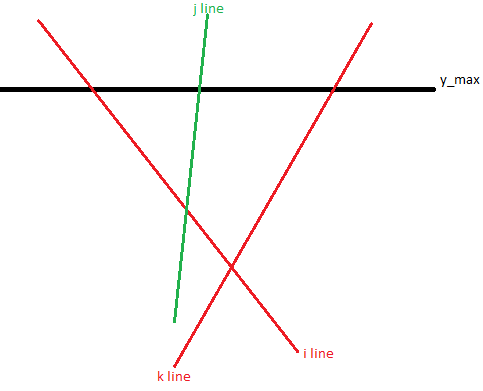
\includegraphics[height=3in]{hw2prob8_4_diagram.png}
\caption{The above argument with the $i,j,k$ lines illustrated}
\end{figure} 

\subsection*{Problem 8.14}

Let S be a set of n points in the plane. Give an O($n^2$) time algorithm to
find the line containing the maximum number of points in S.
\\
\\
Since a line through a pair of points in the primal plane becomes a vertex in the dual plane, we just have to compute the dual of the points and then compute which vertex has the most number of lines passing through it. 
\\
Here is the algorithm:\\
1. Take the dual of the n points\\
2. Use the arrangment algorithm to find the vertices. \\
3. Find which vertex contains the greatest number of lines. \\
\\
\\
Complexity analysis:\\
Taking the dual will take O(n) time. \\
Computing the arrangement takes O($n^2$) time. \\
Going through the vertices will take O($n^2$) time


%\begin{figure}[H]
%\centering
%\includegraphics[height=4in]{prob1plot.jpg}
%\caption{Probability of Class Labels with decision boundaries marked}
%\end{figure}


\end{document}








